% vim: set tw=78 tabstop=4 shiftwidth=4 aw ai:

\chapter{Proiectarea unui protocol multiparty îmbunătățit în nucleul Linux}
\label{chapter:multiparty}

\section{Protocolul swift multiparty}
\label{sec:multiparty:swift}

Protocolul \textit{swift} este un protocol multiparty generic de transport.
Scopul său principal este de a desemina conținut între peer-ii din swarm.
Practic răspunde la doar o singură cerere: \textit{'Uite aici hash-ul!
Dă-mi datele pentru el!}. Entități ca mediile de stocare, servere și
conexiuni sunt abstractizate și sunt invizibile la nivelul API-ului.
Dându-se un hash, datele sunt primite de la oricare sursă dispoinibilă
și integritatea lor este verificată criptografic folosind arbori hash
Merkle~\cite{merkle}.

Mare parte din facilitățile oferite de protocolul \textit{swift} sunt
definite de funcția sa de protocol de transport multiparty centrat pe
conținut. O diferență seminificativă între \textit{swift} și protocolul TCP
este faptul că TCP nu deține nici o informație despre datele pe care le
transportă când datele sunt primite din user-space, pe când protocolul
\textit{swift} are date stabilite anterior și mulți peer-i participă la
distribuirea aceluiași set de date. Din acest motiv și din cauza faptului
că pentru protocolul \textit{switf} ordinea recepționării informației are
puțină importantă, iar absența unui flux fiabil este componsată de redundanță,
renunță la abstractizarea TCP de livrare de flux de date fiabil.
Spre exemplu, datele ,,out-of-order'' vor putea fi în continuare salvate și
aceeași piesă se poate obține de la alt peer.

Principalul nostru obiectiv este integrarea protocolului \textit{swift} ca
un protocol de transport în stiva de rețea din nucleul Linux. Acest lucru
va crește semnificativ performanța transferurilor de date. Dorim să facem
acest lucru cu o intruziune minimă asupra nucleului Linux și modificând cât
mai puțin implementarea actuală de \textit{swift}. Un alt scop este de crea
un API transparent între nucleu și user-space. Un dezvoltator va folosi o
interfață de tip socket pentru a construi o aplicație peste protocolul
\textit{swift}. Pentru a îndeplini acest scop, am implementat un pas
intermediar. Am simulat bucata din kernel în user-space folosind sockeți
raw. Acest lucru are avantajul de a pune la dispoziție o metodă modulară de
a testa funcționalitățile.

\section{Proiectarea unui protocol multiparty}
\label{sec:multiparty:design}

În proiectarea sistemul nostru, am încercat diverse idei, fiecare cu
avantajele și dezavantajele ei. Vom prezenta unele dintre ideile
preliminare ce au condus la alegerea variantei finale.

Prima abordare la care ne-am gândit a fost să includem toate componentele
protocolului swift în nucleu. Acest lucru avea avantajul simplității și ar
fi însemnat un minim de schimbări în arhitectură. Implementarea actuală de
user space putea fi portată ca un modul de kernel.

Deși simplă, această abordare nu putea fi implementată din cauza
restricțiilor de mărime a memoriei în kernel. Pentru testul de integritate,
protocolul swift folosește arbore de hash Merkle. Păstarea acestui arbore
în memoria nucleului nu este scalabilă. Conținutul de pe Internet este mult
prea mare pentru a fi stocat în kernel space. Chiar dacă arborele reține
doar hash-urile datelor deseminate, spațiul tot este insuficient.

Figura~\ref{fig:multiparty:architecture-overview} prezintă principalele module
conceptuale: modulul aplicație, biblioteca de tip \textit{wrapper}, rețeaua de
tip overlay pentru descopeirea peer-ilor și nivelul de protocol de transport.

\begin{figure}
  \centering
  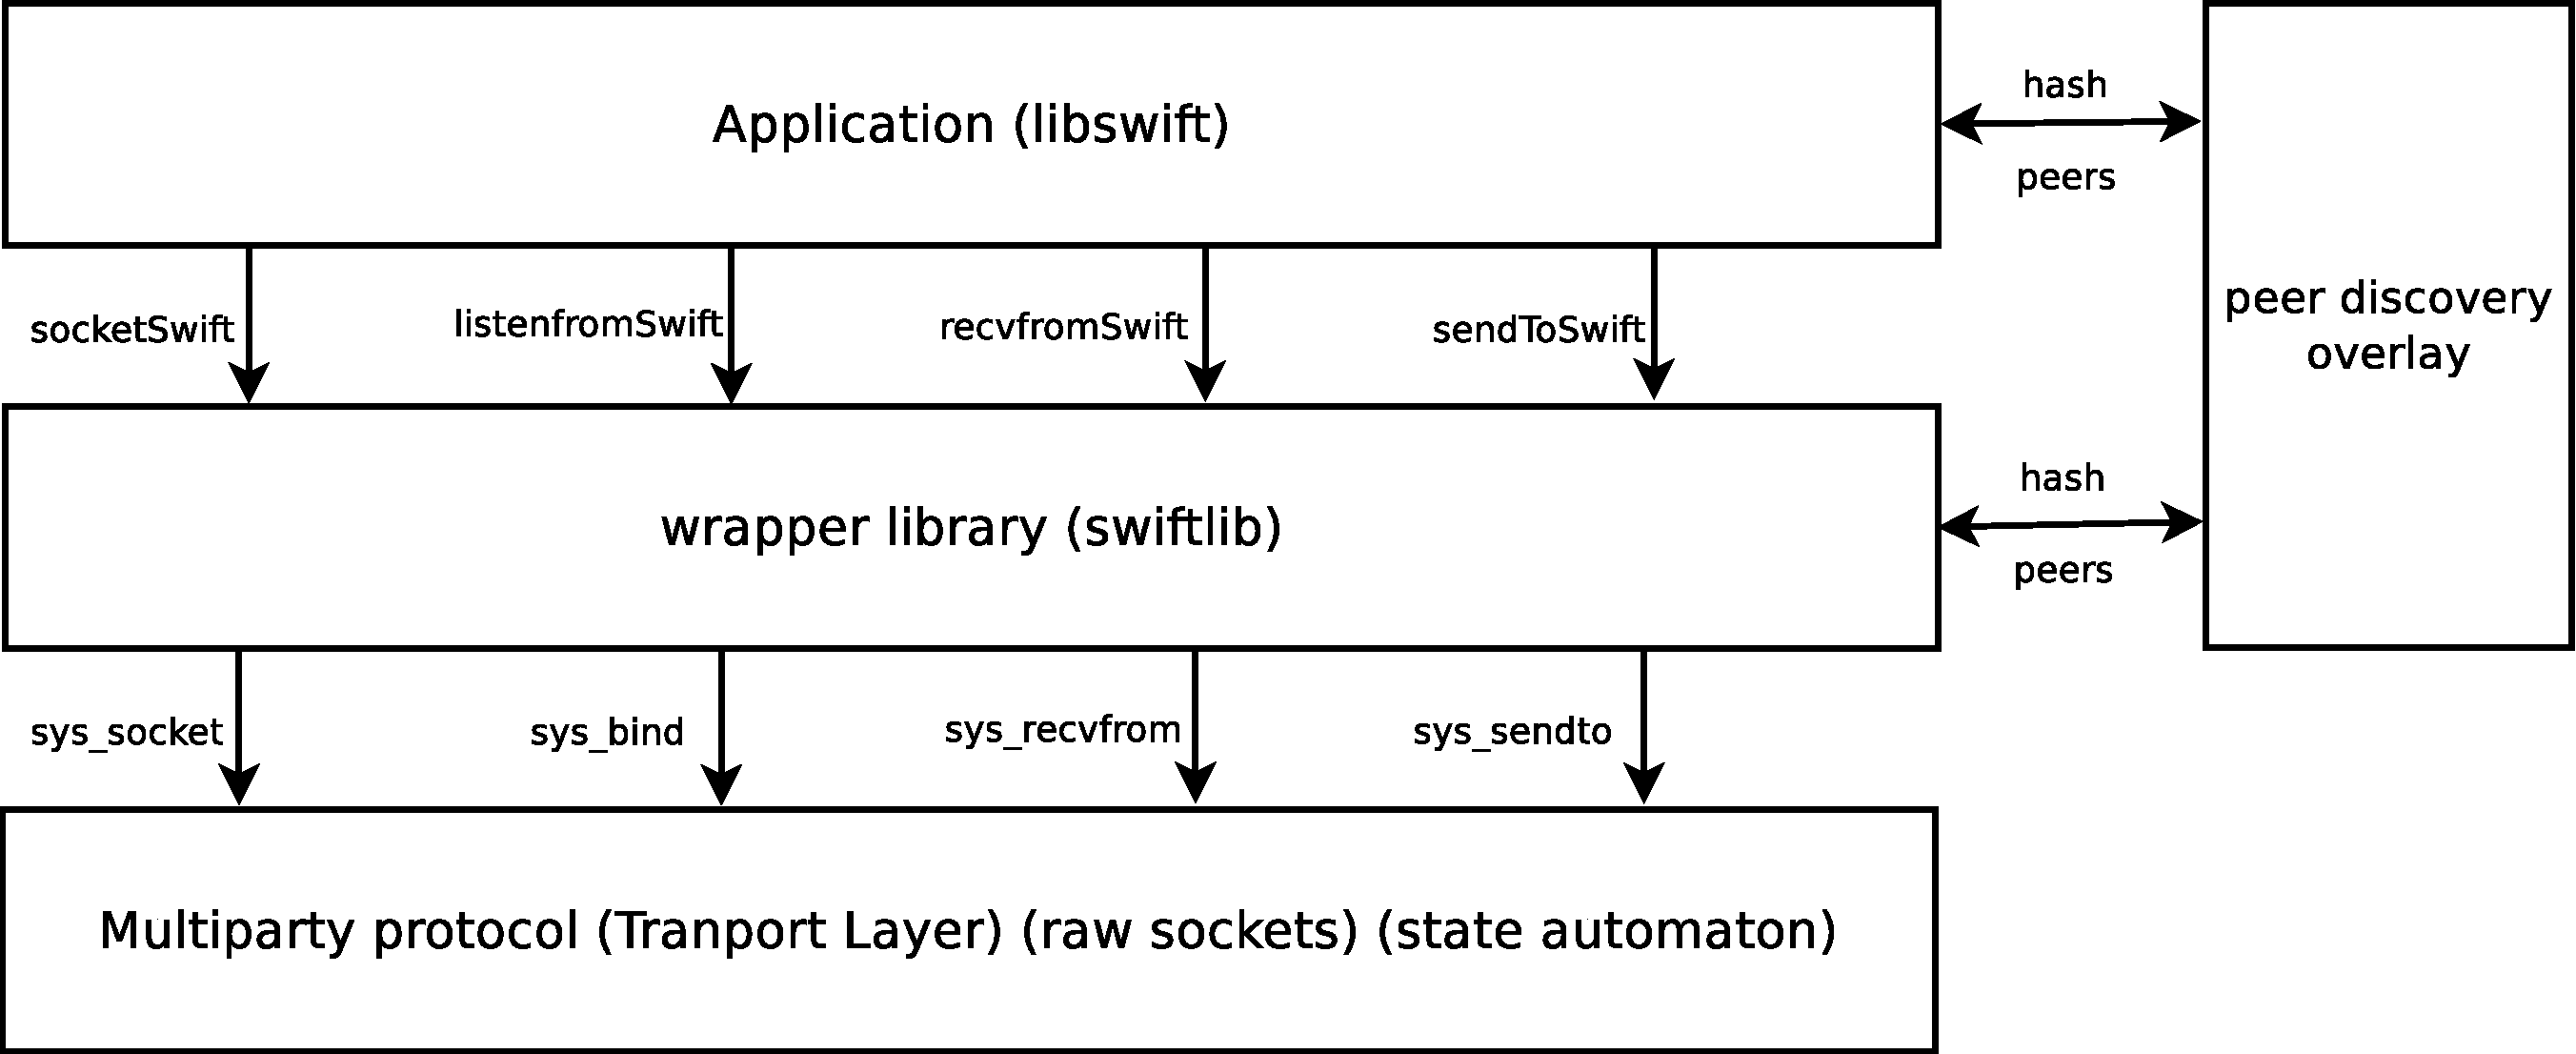
\includegraphics[width=0.6\textwidth]{src/img/multiparty/architecture-overview}
  \caption{Arhitectură sockeți raw}
  \label{fig:multiparty:architecture-overview}
\end{figure}

Modulul aplicație reprezintă partea rămasă din fosta implementare swift. Aceasta
este partea care rămâne în spațiul utilizator și care conține facilități de
gestiunea a fișierelor și a hash-urilor.

Interfața bibliotecii definește un API compatibil cu cel de sockeți pentru
aplicații în spațiul utilizator. Un program va folosi acele apeluri în locul
apelurilor obșinuite de sockeți pentru a beneficia de implementarea
multiparty. Pe moment, aceste apeluri sunt apeluri de sistem simulate care
sunt inițial rezolvate cu ajutorul implementării de sockeți raw. În viitor,
această bibliotecă va reprezenta punctele de intrare în kernel.

Rețeaua de tip overlay pentru descoperirea peer-ilor rămâne neschimbată. Va
continua să funcționeze pe baza sockeților UDP și să lege aceleași niveluri
din implementarea swift ca înainte. Descoperirea peer-ilor va face parte din
implementarea aplicației și va fi alegerea dezvoltatorilor pentru a alege ce
anume trebuie implementat și ce nu.

\section{Implementarea unei interfețe peste sockeți raw}
\label{sec:multiparty:raw-socket}

Protocolul multiparty este implementat pe moment la nivelul utilizator
folosind un nivel de sockeți raw care să valideze arhitectura. Acest lucru are
avantajul simulării unei modularizări a proiectării și permite, de asemenea, o
depanare mai ușoară și o procedură mai simplă de testare a integrării. În
cadrul pasului următor, această parte va fi reprezentată de un patch la
nivelul nucleului care va comunica cu un set de apeluri dedicate prin
intermediul bibliotecii de tip wrapper. Aceste două faze sunt descrise în
Figura~\ref{fig:multiparty:detailed-architecture}.

\begin{figure}
  \centering
  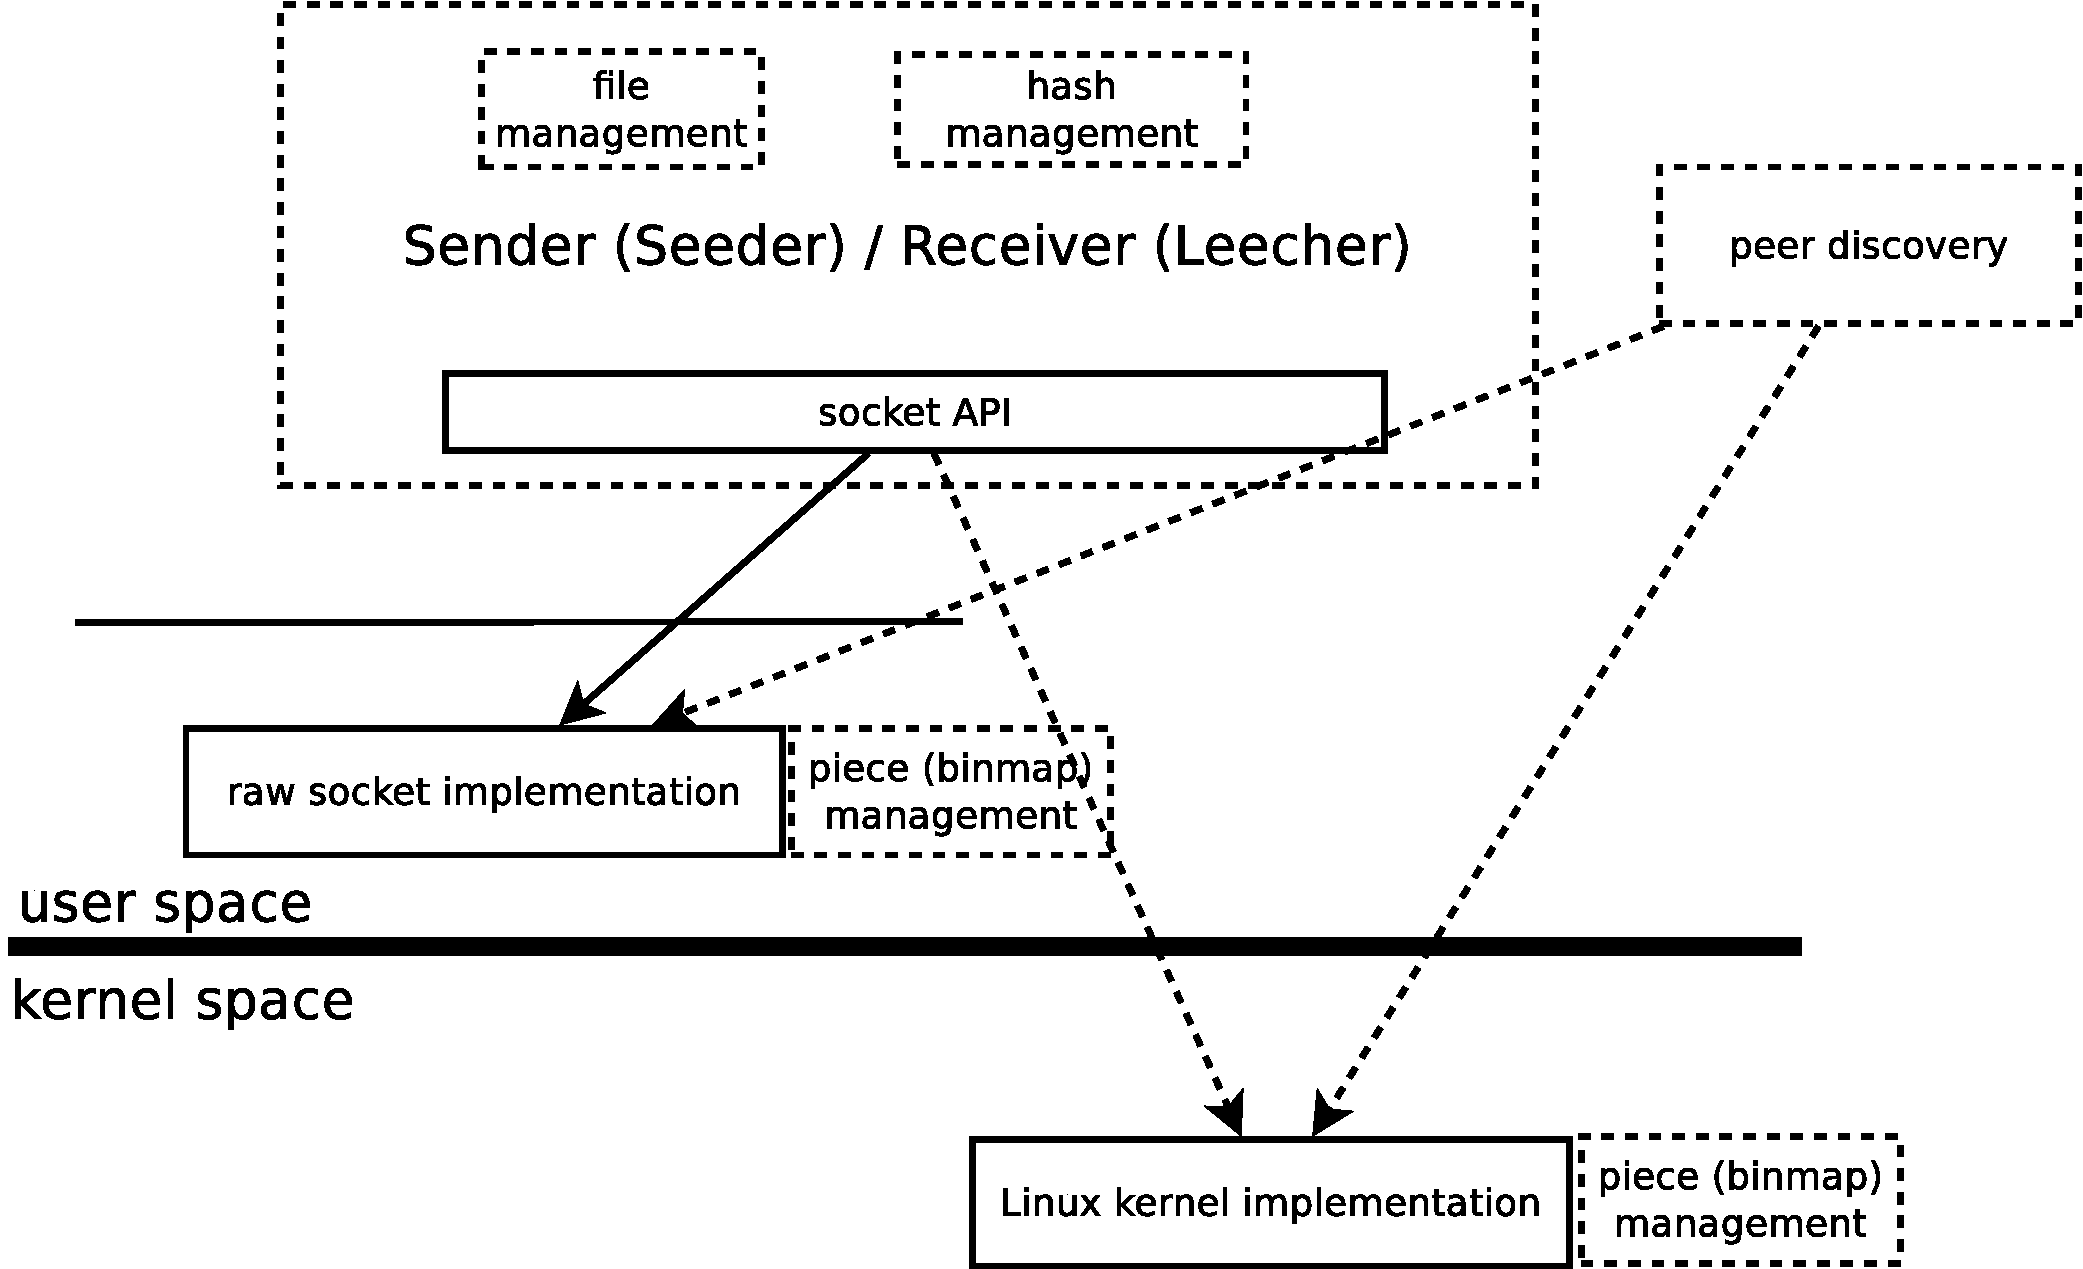
\includegraphics[width=0.6\textwidth]{src/img/multiparty/detailed-architecture}
  \caption{Arhitectură detaliată}
  \label{fig:multiparty:detailed-architecture}
\end{figure}

\begin{figure}
  \centering
  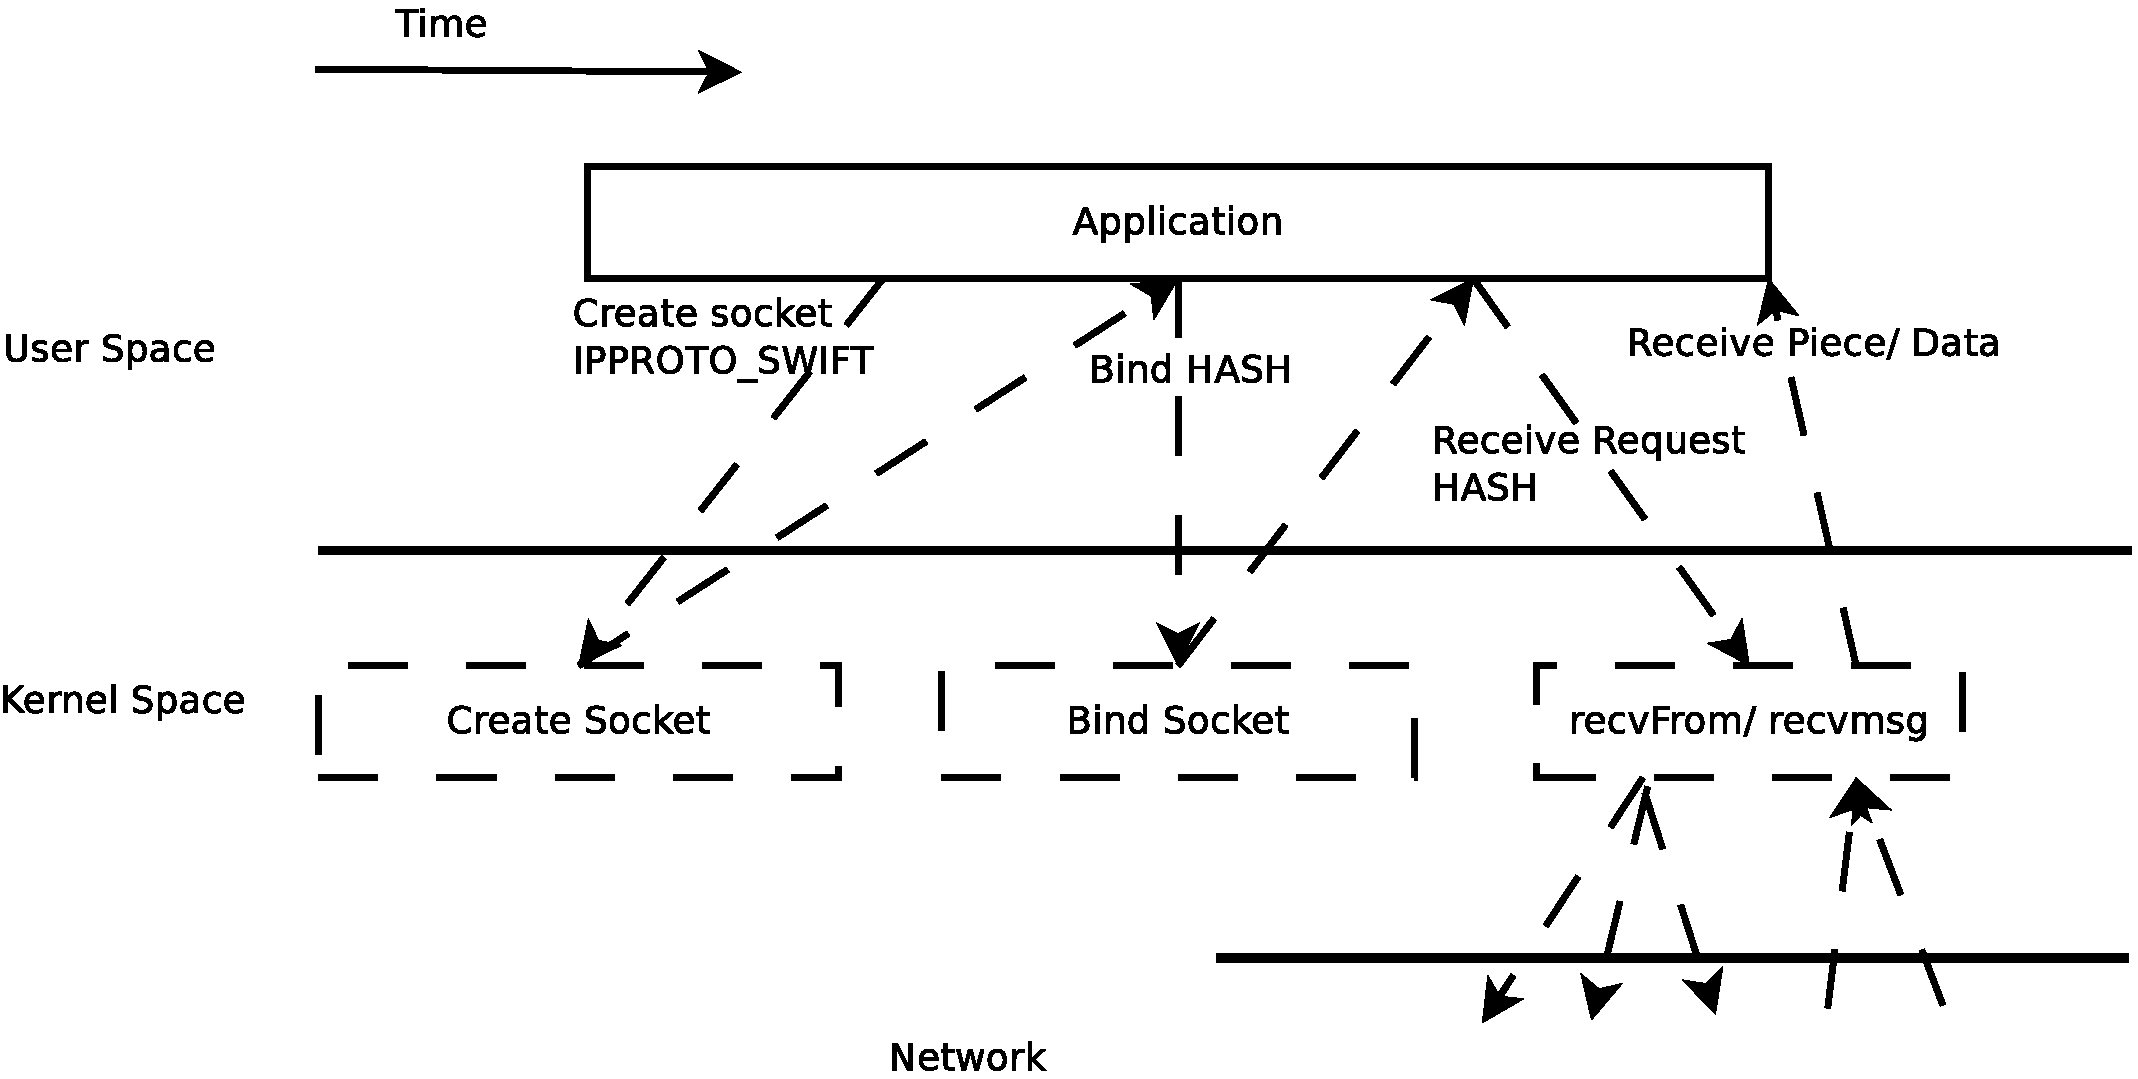
\includegraphics[width=0.55\textwidth]{src/img/multiparty/multiparty-recvmsg}
  \caption{Modelul conceptual al receptorului}
  \label{fig:multiparty:multiparty-recvmsg}
\end{figure}

Figura~\ref{fig:multiparty:multiparty-recvmsg} prezintă modelul conceptual al
unui leecher. Un leecher este peer-ului care solicită informație. Pentru a
realiza acest lucru, trebuie să se conecteze la la protocolul multiparty prin
crearea și inițializarea unui socket. Inițializarea la socket presupune
folosirea unui hash ca parametru pentru a găsi o conexiune cu un peer care
accesează respectivul fișier. Această descoperire este realizată prin
intermediul rețelei de descoperire de tip overlay. Leecher-ul apoi așteaptă
pachete din partea seeder-ului.

\begin{figure}
  \centering
  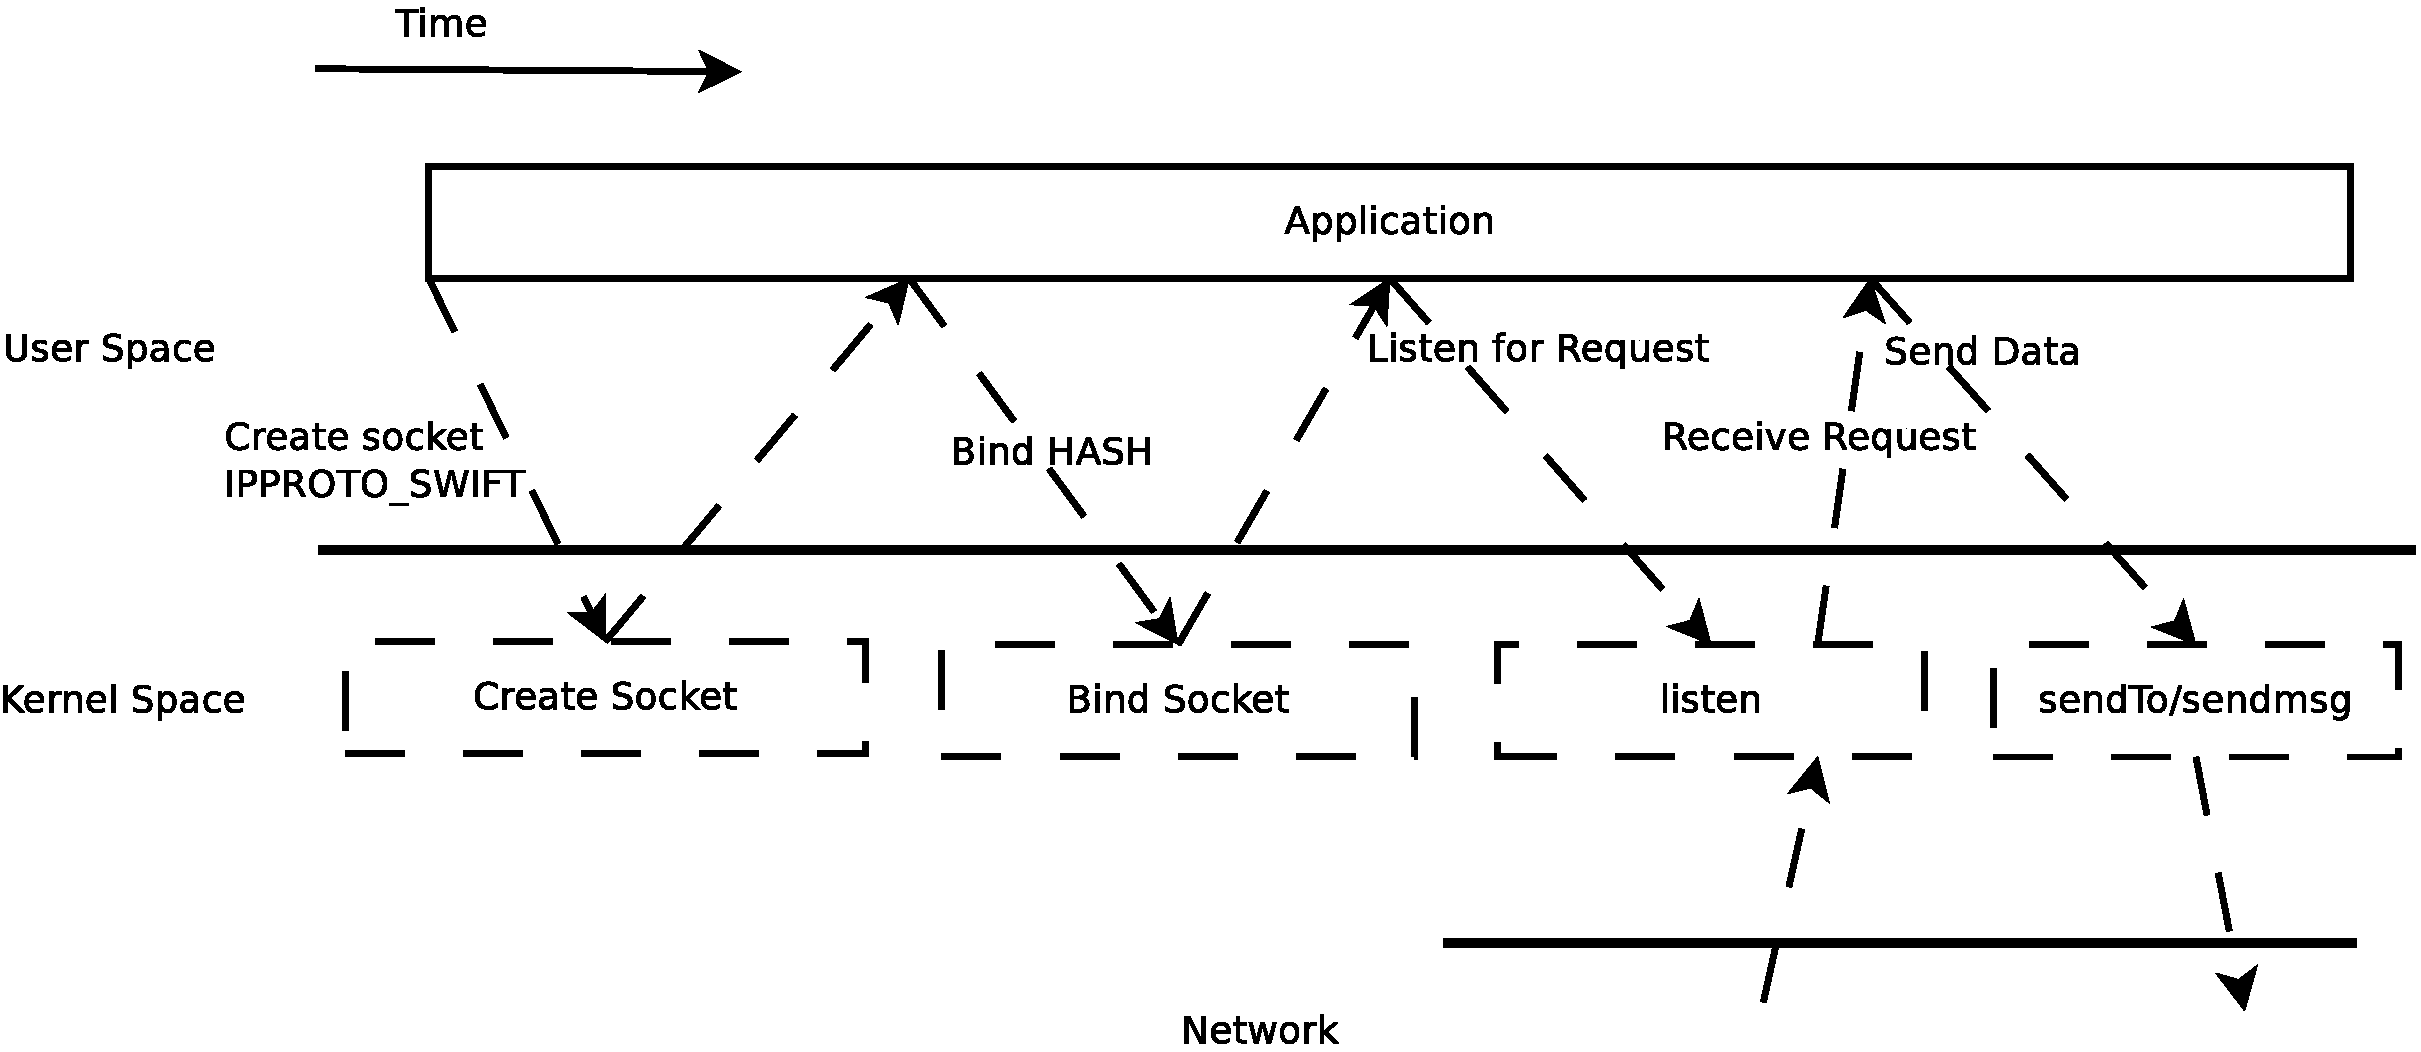
\includegraphics[width=0.55\textwidth]{src/img/multiparty/multiparty-sendmsg}
  \caption{Modelul conceptual al transmițătorului}
  \label{fig:multiparty:multiparty-sendmsg}
\end{figure}

Figura~\ref{fig:multiparty:multiparty-sendmsg} prezintă modelul conceptual al
seeder-ului. Seeder-ul este peer-ul care servește informația către leecheri.
Pentru a realiza acest lucru, se conectează la protocolul multiparty prin
crearea, inițializarea unui socket și apoi ascultarea de conexiuni. La
inițializare, seeder-ul folosește hash-ul ca parametru. Acest lucru înseamnă
că pentru fiecare fișier rezumat va exista un socket pe care seeder-ul va
putea recepționa și servi cereri. Seeder-ul așteaptă conexiuni și transmite
pachete de date conform solicitărilor.

Protocolul este un protocol multiparty generic. Misiunea sa este de a disemina
conținut între peer-ii unui swarm. Fiind dat un hash, datele sunt recepționate
din orice sursă disponibilă iar integritatea datelor este verificată
criptografic cu ajutorul arborilor hash Merkle.

Principala preocupare în modificarea implementări swift este să aibă impact
asupra performanței temporale. În cadrul unui protocol de comunicație, latența
cea mai mare este, în general, generată de așteptarea rezultatelor de la
rețea. Modelul de domunicare multiparty ține cont de acest lucru; următorul
punct de atenție îl reprezintă timpul de rulare a aplicației. Acest lucru este
realizat prin descreșterea penalităților de timp datorate schimbărilor de
context între spațiul utilizator și spațiul kernel. Ideea principală este să
reducem numărul de apeluri de sistem realizate din spațiul utilizator în
spațiul kernel, lucru care va reduce și numărul de schimbări de context.

Interfața de programare pusă la dispoziție este evalută prin intermediul unei
suite de test. Suita de test este implementată folosind vectori de pointeri de
funcții sau structuri cu pointeri de funcții.  O structură de nivel înalt
definește suitele de test pentru fiecare funcție exportată de implementare.
Fiecare suită de test este o serie de metode care testează o formă de apel
al unei funcții.

\section{Framework pentru implementarea protocolului multiparty la nivelul
nucelului}
\label{sec:multiparty:kernel-framework}

Introducerea protocolului multiparty la nivelul nucleului Linux este o
provocare, datorată în principal particularităților sale față de implementări
obișnuite de protocol. Un protocol de transport multiparty folosește puncte
multiple într-o comunicație, spre deosebire de protocoalele tradiționale de
comunicație care permit un singur transmițător și un singur receptor.

Pentru a implementa un protocol de nivel transport în nucleul Linux, câteva
faze de design trebuie să fie îndeplinite:

\begin{itemize}
  \item Definirea \texttt{IPPROTO\_\$\$}. Acest macro va identifica protocolul
  de nivel transport. Acesta va fi ulterior folosit pentru a crea un socket de
  nivel transport.
  \item Definirea unui header de nivel transport. Framework-ul pe care l-am
  folosit definește două porturi de 8 biți, un port sursă și unul destinație
  și un câmp cu lungimea de 16 biți. Cel din urmă este lungimea datelor,
  incluzând header-ul de nivel transport.
\end{itemize}

După realizarea fazelor de mai sus, trebuie definite structurile relevante, ca
mai jos.

Trebuie definită o structură pentru tipul de socket. Aceasta este structura în
care trebuie să se afle informație legată de starea socket-ului, precum portul
sursă și portul destinație.

\begin{verbatim}
struct swift_sock {
    struct inet_sock sock;
    /* swift socket speciffic data */
    uint8_t src;
    uint8_t dst;
};
\end{verbatim}

Definiția protocolului, folosită de socket, incluzând numele și dimensiunea sa
se găsesc în cadrul structurii \texttt{struct proto}.

\begin{verbatim}
static struct proto swift_prot = {
    .obj_size = sizeof(struct swift_sock),
    .owner = THIS_MODULE,
    .name = "SWIFT",
};
\end{verbatim}

Cea mai importantă structură care să fie definită descrie operațiile care vor
fi implementate pentru un socket de un tip dat. Pentru socket care trimite
datagrame, implementarea funcțiilor \texttt{release}, \texttt{connect},
\texttt{sendmsg} și \texttt{recvmsg} este suficientă.

Header-ul pentru noile pachete este construit în cadrul unei structuri de
tipul \texttt{net\_protocol}. Noile pachete, care sunt recepționate direct de
la rețea, vor completa câmpul \texttt{protocol} în header-ul IP cu valoarea
implementată de protocolul de nivelul transport.

Înainte de compilarea și inserarea modulului în nucleu, câteva operații pe
sockeți trebuie să fie implementate; pentru swift (un protocol bazat pe
datagrame), aceasta înseamnă \texttt{release}, \texttt{bind}, \texttt{connect},
\texttt{sendmsg} și \texttt{recvmsg}. Un handler de pachete recepționate din
rețea trebuie să fie, de asemenea, implementat. La nivelul protocolului
trebuie realizată o mapare între port și socket, însemnând că socket-ul este
inițializat cu acel port.

La fel ca în cazul implementării peste sockeți raw, o suită de teste unitare a
fost implementată. În cadrul acestei suite, unele teste sunt simple, care să
asigure funcționalitate de bază, iar un set de alte teste sunt folosite pentru a
verifica valorile de eroare întoarse și performanța protocolului. Performanța
protocolului este corelată cu asigurarea scalabilității -- conexiuni de
client muliple și simultane.

Testarea funcțională impune o proiectare și implementare a testelor pentru
fiecare funcție expusă de protocol. Altfel spus, există o suită de test pentru
fiecare dintre funcțiile \texttt{bind}, \texttt{connect}, \texttt{close},
\texttt{sendto}, \texttt{recvfrom}, \texttt{sendmsg}, \texttt{recvmsg},
\texttt{send} and \texttt{recv}. Suitele de teste sunt portări ale suitelor
de test pentru sockeți raw. Datorită similarității interfeței furnizate de
implementarea cu sockeți raw și cea de la nivelul nucleului, portarea este
facilă.
